Global Arrays provide functions for collective array operations, targeting
both whole arrays and patches (portions of global arrays). Collective
operations require all the processes to make the call. In the underlying
implementation, each process deals with its local data. These functions
include:
\begin{itemize}
\item basic array operations, 
\item linear algebra operations, and 
\item interfaces to third party software packages.
\end{itemize}

\section{Basic Array Operations }

Global Arrays provide several mechanisms to manipulate contents of
the arrays. One can set all the elements in an array/patch to a specific
value, or as a special case set to zero. Since GA does not explicitly
initialize newly created arrays, these calls are useful for initialization
of an array/patch. (To fill the array with different values for each
element, one can choose the one sided operation putor each process
can initialize its local portion of an array/patch like ordinary local
memory). One can also scale the array/patch by a certain factor, or
copy the contents of one array/patch to another. 


\subsection{Whole Arrays }

These functions apply to the entire array.

The function
\begin{lyxcode}
\textcolor{blue}{Fortran}~subroutine~\href{http://www.emsl.pnl.gov/docs/global/ga_ops.html\#ga_zero}{ga\_{}zero}(g\_a)~

\textcolor{blue}{C}~~~~~~~void~\href{http://www.emsl.pnl.gov/docs/global/c_nga_ops.html\#ga_zero}{GA\_{}Zero}(int~g\_a)~

\textcolor{blue}{C++}~~~~~void~GA::GlobalArray::zero()
\end{lyxcode}
sets all the elements in the array to zero.

To assign a single value to all the elements in an array, use the
function
\begin{lyxcode}
\textcolor{blue}{Fortran}~subroutine~\href{http://www.emsl.pnl.gov/docs/global/ga_ops.html\#ga_fill}{ga\_{}fill}(g\_a,~val)~

\textcolor{blue}{C}~~~~~~~void~\href{http://www.emsl.pnl.gov/docs/global/c_nga_ops.html\#ga_fill}{GA\_{}Fill}(int~g\_a,~void~{*}val)~

\textcolor{blue}{C++}~~~~~void~GA::GlobalArray::fill(void~{*}val)
\end{lyxcode}
It sets all the elements in the array to the value \emph{val}. The
\emph{val} must have the same data type as that of the array.

The function
\begin{lyxcode}
\textcolor{blue}{Fortran}~subroutine~\href{http://www.emsl.pnl.gov/docs/global/ga_ops.html\#ga_scale}{ga\_{}scale}(g\_a,~val)~

\textcolor{blue}{C}~~~~~~~void~\href{http://www.emsl.pnl.gov/docs/global/c_nga_ops.html\#ga_scale}{GA\_{}scale}(int~g\_a,~void~{*}val)~

\textcolor{blue}{C++}~~~~~void~GA::GlobalArray::scale(void~{*}val)
\end{lyxcode}
scales all the elements in the array by factor \emph{val}. Again the
val must be the same data type as that of the array itself.

The above three functions are dealing with one global array, to set
values or change all the elements together. The following functions
are for copying data between two arrays.

The function
\begin{lyxcode}
\textcolor{blue}{Fortran}~subroutine~\href{http://www.emsl.pnl.gov/docs/global/ga_ops.html\#ga_copy}{ga\_{}copy}(g\_a,~g\_b)~

\textcolor{blue}{C}~~~~~~~void~\href{http://www.emsl.pnl.gov/docs/global/c_nga_ops.html\#ga_copy}{GA\_{}copy}(int~g\_a,~int~g\_b)~

\textcolor{blue}{C++}~~~~~void~GA::GlobalArray::copy

~~~~~~~~~~~~~(const~GA::GlobalArray~{*}~g\_a)
\end{lyxcode}
copies the contents of one array to another. The arrays must be of
the same data type and have the same number of elements.

For global arrays containing ghost cells, the ghost cell data can
be filled in with the corresponding data from neighboring processors
using the command
\begin{lyxcode}
\textcolor{blue}{n-d~Fortran}~subroutine~\href{http://www.emsl.pnl.gov/docs/global/ga_ops.html\#ga_copy}{ga\_{}copy}(g\_a,~g\_b)~

\textcolor{blue}{C~}~~~~~~~~~~void~\href{http://www.emsl.pnl.gov/docs/global/c_nga_ops.html\#ga_copy}{GA\_{}copy}(int~g\_a,~int~g\_b)~

\textcolor{blue}{C++}~~~~~~~~~void~GA::GlobalArray::

~~~~~~~~~~~~~~~~~~copy(const~GA::GlobalArray~{*}~g\_a)



\textcolor{blue}{n-d~Fortran}~subroutine~\href{http://www.emsl.pnl.gov/docs/global/ga_ops.html\#ga_update_ghosts}{ga\_{}update\_{}ghosts}(g\_a)~

\textcolor{blue}{C}~~~~~~~~~~~void~\href{http://www.emsl.pnl.gov/docs/global/c_nga_ops.html\#ga_update_ghosts}{ga\_{}update\_{}ghosts}(int~g\_a)~

\textcolor{blue}{C++}~~~~~~~~~void~GA::GlobalArray::updateGhosts()~
\end{lyxcode}
This operation updates the ghost cell data by assuming periodic, or
wrap-around, boundary conditions similar to those described for the\texttt{
nga\_periodic\_get} operations described above. The wrap-around conditions
are always applied, it is up to the individual application to decide
whether or not the data in the ghost cells should be used. The update
operation is illustrated below for a simple 4x2 global array distributed
across two processors. The ghost cells are one element wide in each
dimension.

\begin{tabular}{|c|}
\hline 
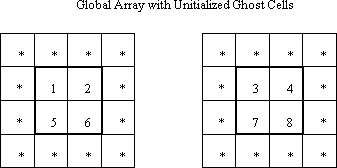
\includegraphics[width=10cm]{ghost012}\tabularnewline
\hline
\hline 
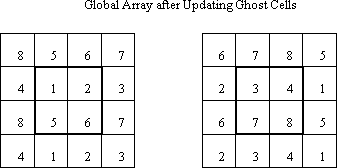
\includegraphics[width=10cm]{ghost015}\tabularnewline
\hline
\end{tabular}
\begin{lyxcode}
\textcolor{blue}{n-d~Fortran}~logical~function~\href{http://www.emsl.pnl.gov/docs/global/ga_ops.html\#ga_update_ghost_dir}{nga\_{}update\_{}ghosts\_{}dir}(g\_a,~

~~~~~~~~~~~~~~~~~~~~~~~~dimension,~idir,~flag)~

\textcolor{blue}{C}~~~~~~~~~~~int~\href{http://www.emsl.pnl.gov/docs/global/c_nga_ops.html\#nga_update_ghost_dir}{NGA\_{}Update\_{}ghosts\_{}dir}(int~g\_a,~int~

~~~~~~~~~~~~~~~~~~~~~~~~dimension,~int~idir,~int~cflag)~

\textcolor{blue}{C++}~~~~~~~~~int~GA::GlobalArray::updateGhostsDir

~~~~~~~~~~~~~~~~~~~~~~~(int~dimension,~int~idir,~int~cflag)~
\end{lyxcode}
This function can be used to update the ghost cells along individual
directions.

It is designed for algorithms that can overlap updates with computation.
The variable dimension indicates which coordinate direction is to
be updated (e.g. dimension = 1 would correspond to the y axis in a
two or three dimensional system), the variable idir can take the values
+/-1 and indicates whether the side that is to be updated lies in
the positive or negative direction, and cflag indicates whether or
not the corners on the side being updated are to be included in the
update. The following calls would be equivalent to a call to \texttt{GA\_Update\_ghosts}
for a 2-dimensional system:
\begin{lyxcode}
status~=~NGA\_Update\_ghost\_dir(g\_a,0,-1,1);~

status~=~NGA\_Update\_ghost\_dir(g\_a,0,1,1);~

status~=~NGA\_Update\_ghost\_dir(g\_a,1,-1,0);~

status~=~NGA\_Update\_ghost\_dir(g\_a,1,1,0);
\end{lyxcode}
The variable \emph{cflag} is set equal to 1 (or non-zero) in the first
two calls so that the corner ghost cells are update, it is set equal
to 0 in the second two calls to avoid redundant updates of the corners.
Note that updating the ghosts cells using several independent calls
to the \texttt{nga\_update\_ghost\_dir} functions is generally not
as efficient as using \texttt{GA\_Update\_ghosts} unless the individual
calls can be effectively overlapped with computation. This is a collective
operation. 


\subsection{Patches }

GA provides a set of operations on segments of the global arrays,
namely patch operations. These functions are more general, in a sense
they can apply to the entire array(s). As a matter of fact, many of
the Global Array collective operations are based on the patch operations,
for instance, the \texttt{GA\_Printis} only a special case of \texttt{NGA\_Print\_patch},
called by setting the bounds of the patch to the entire global array.
There are two interfaces for Fortran, one for two dimensional and
the other for n-dimensional (one to seven). The (n-dimensional) interface
can surely handle the two dimensional case as well. It is available
for backward compatibility purposes. The functions dealing with n-dimensional
patches use the \textquotedbl{}\texttt{nga}\textquotedbl{}prefix and
those dealing with two dimensional patches start with the \textquotedbl{}\texttt{ga}\textquotedbl{}
prefix.

The function
\begin{lyxcode}
\textcolor{blue}{Fortran}~subroutine~\href{http://www.emsl.pnl.gov/docs/global/ga_ops.html\#ga_zero_patch}{nga\_{}zero\_{}patch}nga\_zero\_patch(g\_a,~alo,~ahi)~

\textcolor{blue}{C}~~~~~~~void~\href{http://www.emsl.pnl.gov/docs/global/c_nga_ops.html\#ga_zero_patch}{NGA\_{}Zero\_{}patch}(int~g\_a,~int~lo{[}{]}~int~hi{[}{]})~

\textcolor{blue}{C++}~~~~~void~GA::GlobalArray::zeroPatch(int~lo{[}{]}~int~hi{[}{]})
\end{lyxcode}
is similar to \emph{ga\_zero}, except that instead of applying to
entire array, it sets only the region defined by \emph{lo} and \emph{hi}
to zero.

One can assign a single value to all the elements in a patch with
the function:
\begin{lyxcode}
\textcolor{green}{n-D}\textcolor{blue}{Fortran}~subroutine~\href{http://www.emsl.pnl.gov/docs/global/ga_ops.html\#ga_fill_patch}{nga\_{}fill\_{}patch}(g\_a,~lo,~hi,~val)~

\textcolor{green}{2-D}\textcolor{blue}{Fortran}~subroutine~\href{http://www.emsl.pnl.gov/docs/global/ga_ops.html\#ga_fill_patch}{ga\_{}fill\_{}patch}(g\_a,~ilo,~ihi,~

~~~~~~~~~~~~~~~~~~~jlo,~jhi,~val)~

\textcolor{blue}{C}~~~~~~~~~~void~\href{http://www.emsl.pnl.gov/docs/global/c_nga_ops.html\#ga_fill_patch}{NGA\_{}Fill\_{}patch}(int~g\_a,~int~lo{[}{]}~

~~~~~~~~~~~~~~~~~~~int~hi{[}{]},~void~{*}val)~

\textcolor{blue}{C++}~~~~~~~~void~GA::GlobalArray::fillPatch(int~lo{[}{]}~

~~~~~~~~~~~~~~~~~~~int~hi{[}{]},~void~{*}val)
\end{lyxcode}
The\texttt{ lo} and \texttt{hi} defines the patch and the \texttt{val}
is the value to set.

The function
\begin{lyxcode}
\textcolor{green}{n-D}\textcolor{blue}{Fortran}~subroutine~\href{http://www.emsl.pnl.gov/docs/global/ga_ops.html\#ga_scale_patch}{nga\_{}scale\_{}patch}(g\_a,~lo,~hi,~val)~

\textcolor{green}{2-D}\textcolor{blue}{Fortran}~subroutine~\href{http://www.emsl.pnl.gov/docs/global/ga_ops.html\#ga_scale_patch}{ga\_{}scale\_{}patch}(g\_a,~ilo,~ihi,~jlo,~

~~~~~~~~~~~~~~~~~~jhi,~val)~

\textcolor{blue}{C}~~~~~~~~~~void~\href{http://www.emsl.pnl.gov/docs/global/c_nga_ops.html\#ga_scale_patch}{NGA\_{}Scale\_{}patch}(int~g\_a,~int~lo{[}{]}~int~

~~~~~~~~~~~~~~~~~~hi{[}{]},~void~{*}val)~

\textcolor{blue}{C++}~~~~~~~~void~GA::GlobalArray::scalePatch(int~lo{[}{]}~

~~~~~~~~~~~~~~~~~~int~hi{[}{]},~void~{*}val)
\end{lyxcode}
scales the patch defined by \texttt{lo }and \texttt{hi} by the factor
\texttt{val}.

The copy patch operation is one of the fundamental and frequently
used functions. The function
\begin{lyxcode}
\textcolor{green}{n-D}\textcolor{blue}{Fortran}~subroutine~\href{http://www.emsl.pnl.gov/docs/global/ga_ops.html\#ga_copy_patch}{nga\_{}copy\_{}patch}(trans,~g\_a,~alo,~

~~~~~~~~~~~~~~~~~~~~~~ahi,~g\_b,~blo,~bhi)~

\textcolor{green}{2-D}\textcolor{blue}{Fortran}~subroutine~\href{http://www.emsl.pnl.gov/docs/global/ga_ops.html\#ga_copy_patch}{ga\_{}copy\_{}patch}(trans,~g\_a,~ailo,~

~~~~~~~~~~~~~~~~~~~~~~aihi,~ajlo,~ajhi,~g\_b,~bilo,~bihi,~

~~~~~~~~~~~~~~~~~~~~~~bjlo,~bjhi)~

\textcolor{blue}{C~}~~~~~~~~~void~\href{http://www.emsl.pnl.gov/docs/global/c_nga_ops.html\#ga_copy_patch}{NGA\_{}Copy\_{}patch}(char~trans,~int~g\_a~,~

~~~~~~~~~~~~~~~~~~~~~~int~alo{[}{]},~int~ahi{[}{]},~int~g\_b,~

~~~~~~~~~~~~~~~~~~~~~~int~blo{[}{]},~int~bhi{[}{]})~

\textcolor{blue}{C++}~~~~~~~~voidGA::GlobalArray::copyPatch(char~trans,~

~~~~~~~~~~~~~~~~~~~~~~const~GA::GlobalArray{*}~g\_a,~int~alo{[}{]},~

~~~~~~~~~~~~~~~~~~~~~~int~ahi{[}{]},~int~blo{[}{]},~int~bhi{[}{]})
\end{lyxcode}
copies one patch defined by \texttt{alo} and \texttt{ahi} in one global
array \texttt{g\_ato} another patch defined by \texttt{blo} and \texttt{bhi}
in another global array \texttt{g\_b}. The current implementation
requires that the source patch and destination patch must be on different
global arrays. They must also be the same data type. The patches may
be of different shapes, but the number of elements must be the same.
During the process of copying, the transpose operation can be performed
by specifying trans.

\emph{Example}: Assume that there two 8x6 Global Arrays, \texttt{g\_a}
and \texttt{g\_b},distributed on three processes. The operation of
\texttt{nag\_copy\_patch}(Fortran notation), from
\begin{lyxcode}
g\_a:~alo~=~\{2,~2\},~ahi~=~\{4,~5\}
\end{lyxcode}
to
\begin{lyxcode}
g\_b:~blo~=~\{3,~4\},~bhi~=~\{6,~6\}
\end{lyxcode}
and
\begin{lyxcode}
trans~=~0
\end{lyxcode}
involves reshaping. It is illustrated in the following figure. 

\begin{tabular}{|c|}
\hline 
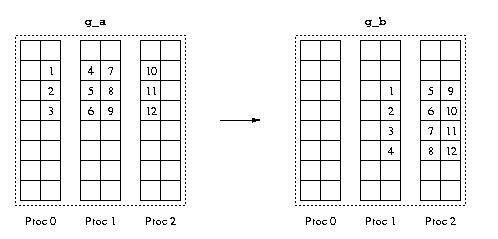
\includegraphics[width=10cm]{copy1}\tabularnewline
\hline
\end{tabular}

One step further, if one also want to perform the transpose operation
during the copying, i.e. set \texttt{\textcolor{black}{trans = 1}},
it will look like: 

\begin{tabular}{|c|}
\hline 
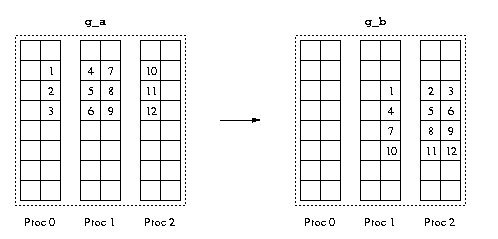
\includegraphics[width=10cm]{copy2}\tabularnewline
\hline
\end{tabular}

If there is no reshaping or transpose, the operation can be fast (internally
calling \texttt{nga\_put}). Otherwise, it would be slow (internally
calling \texttt{nga\_scatter}, where extra time is spent on preparing
the indices). Also note that extra memory is required to hold the
indices if the operation involves reshaping or transpose. 


\section{Linear Algebra }

Global arrays provide three linear algebra operations: addition, multiplication,
and dot product. There are two sets of functions, one for the whole
array and the other for the patches. 


\subsection{Whole Arrays }

The function
\begin{lyxcode}
\textcolor{blue}{Fortran}~subroutine~\href{http://www.emsl.pnl.gov/docs/global/ga_ops.html\#ga_add}{ga\_{}add}(alpha,~g\_a,~beta,~g\_b,~g\_c)~

\textcolor{blue}{C}~~~~~~~void~\href{http://www.emsl.pnl.gov/docs/global/c_nga_ops.html\#ga_add}{GA\_{}Add}(void~{*}alpha,~int~g\_a,~

~~~~~~~~void~{*}beta,int~g\_b,~int~g\_c)~

\textcolor{blue}{C++}~void~GA::GlobalArray::add(void~{*}alpha,~~

~~~~~~~~const~GA::GlobalArray{*}~g\_a,~

~~~~~~~~void~{*}beta,~const~GA::GlobalArray{*}~g\_b)
\end{lyxcode}
adds two arrays, \texttt{g\_a} and \texttt{g\_b}, and saves the results
to \texttt{g\_c}. The two source arrays can be scaled by certain factors.
This operation requires the two source arrays have the same number
of elements and the same data types, but the arrays can have different
shapes or distributions.\texttt{ g\_c} can also be \texttt{g\_a} or
\texttt{g\_b}. It is encouraged to use this function when the two
source arrays are identical in distributions and shapes, because of
its efficiency. It would be less efficient if the two source arrays
are different in distributions or shapes.

Matrix multiplication operates on two matrices, therefore the array
must be two dimensional. The function
\begin{lyxcode}
\textcolor{blue}{Fortran}~subroutine~\href{http://www.emsl.pnl.gov/docs/global/ga_ops.html\#ga_dgemm}{ga\_{}dgemm}(transa,~transb,~m,~n,~k,~

~~~~~~~~~~~~~~alpha,~g\_a,~g\_b,~beta,~g\_c~)~

\textcolor{blue}{C}~~~~~~~void~\href{http://www.emsl.pnl.gov/docs/global/c_nga_ops.html\#ga_dgemm}{GA\_{}Dgemm}(char~ta,~char~tb,~int~m,~int~n,~

~~~~~~~~~~~~~~int~k,~double~alpha,~int~g\_a,~int~g\_b,~

~~~~~~~~~~~~~~double~beta,~int~g\_c~)~

\textcolor{blue}{C++}~~~~~void~GA::GlobalArray::dgemm(char~ta,~char~tb,~

~~~~~~~~~~~~~~int~m,~int~n,~int~k,~double~alpha,~

~~~~~~~~~~~~~~const~GA::GlobalArray{*}~g\_a,~const~GA::GlobalArray{*}~

~~~~~~~~~~~~~~g\_b,~double~beta)
\end{lyxcode}
Performs one of the matrix-matrix operations:

\emph{C := alpha{*}op( A ){*}op( B ) + beta{*}C,}

where op( X ) is one of

\emph{op( X ) = X or op( X ) = X',}

alpha and beta are scalars, and \emph{A}, \emph{B,} and \emph{C} are
matrices, with \emph{op( A ) }an \emph{m} by \emph{k} matrix, \emph{op(
B )} a \emph{k} by \emph{n} matrix and \emph{C} an \emph{m} by \emph{n}
matrix.

On entry, transa specifies the form of \emph{op( A )} to be used in
the matrix multiplication as follows: 

\emph{ta = 'N'} or\emph{ 'n', op( A ) = A}. 

\emph{ta = 'T'} or \emph{'t', op( A ) = A'}.

The function
\begin{lyxcode}
Fortran~integer~function~ga\_idot(g\_a,~g\_b)~

~~~~~~~~double~precision~function~\href{http://www.emsl.pnl.gov/docs/global/ga_ops.html\#ga_ddot}{ga\_{}ddot}(g\_a,~g\_b)

~~~~~~~~double~complex~function~\href{http://www.emsl.pnl.gov/docs/global/ga_ops.html\#ga_zdot}{ga\_{}zdot}(g\_a,~g\_b)~

C~~~~~~~long~\href{http://www.emsl.pnl.gov/docs/global/c_nga_ops.html\#ga_dot}{GA\_{}Idot}(int~g\_a,~int~g\_b)~

~~~~~~~~double~G\href{http://www.emsl.pnl.gov/docs/global/c_nga_ops.html\#ga_dot}{GA\_{}Ddot}A\_Ddot(int~g\_a,~int~g\_b)~

~~~~~~~~DoubleComplex~\href{http://www.emsl.pnl.gov/docs/global/c_nga_ops.html\#ga_dot}{GA\_{}Zdot}GA\_Zdot(int~g\_a,~int~g\_b)~

C++~~~~~long~GA::GlobalArray::idot

~~~~~~~~~~~~~~~~~(const~GA::GlobalArray{*}~g\_a)~

~~~~~~~~double~GA::GlobalArray::ddot

~~~~~~~~~~~~~~~~~(const~GA::GlobalArray{*}~g\_a)~

~~~~~~~~DoubleComplex~GA::GlobalArray::zdot

~~~~~~~~~~~~~~~~~(const~GA::GlobalArray{*}~g\_a)
\end{lyxcode}
computes the element-wise dot product of two arrays. It is available
as three separate functions, corresponding to \emph{integer}, \emph{double
precision} and \emph{double complex} data types.

The following functions apply to the 2-dimensional whole arrays only.
There are no corresponding functions for patch operations.

The function
\begin{lyxcode}
\textcolor{blue}{Fortran}~subroutine~\href{http://www.emsl.pnl.gov/docs/global/ga_ops.html\#ga_symmetrize}{ga\_{}symmetrize}(g\_a)~

\textcolor{blue}{C}~~~~~~~void~\href{http://www.emsl.pnl.gov/docs/global/c_nga_ops.html\#ga_symmetrize}{GA\_{}Symmetrize}(int~g\_a)~

\textcolor{blue}{C++}~~~~~void~GA::GlobalArray::symmetrize()
\end{lyxcode}
symmetrizes matrix A represented with handle \texttt{g\_a}:\emph{A
= .5 {*} (A+A')}.

The function
\begin{lyxcode}
\textcolor{blue}{Fortran}~subroutine~\href{http://www.emsl.pnl.gov/docs/global/ga_ops.html\#ga_transpose}{ga\_{}transpose}(g\_a,~g\_b)~

\textcolor{blue}{C}~~~~~~~void~\href{http://www.emsl.pnl.gov/docs/global/c_nga_ops.html\#ga_transpose}{GA\_{}Transpose}(int~g\_a,~int~g\_b)~

\textcolor{blue}{C++}~~~~~void~GA::GlobalArray::transpose

~~~~~~~~~~~~~(const~GA::GlobalArray{*}~g\_a)
\end{lyxcode}
transposes a matrix: B = A'.


\subsection{Patches }

The functions
\begin{lyxcode}
\textcolor{green}{n-D}\textcolor{blue}{Fortran}~subroutine~\href{http://www.emsl.pnl.gov/docs/global/ga_ops.html\#ga_add_patch}{nga\_{}add\_{}patch}(alpha,~g\_a,~

~~~~~~~~~~~~~~~~~~~~~~alo,~ahi,~beta,~g\_b,~blo,~

~~~~~~~~~~~~~~~~~~~~~~bhi,~g\_c,~clo,~chi)~

\textcolor{green}{2-D}\textcolor{blue}{Fortran}~subroutine~\href{http://www.emsl.pnl.gov/docs/global/ga_ops.html\#ga_add_patch}{ga\_{}add\_{}patch}(alpha,~g\_a,~

~~~~~~~~~~~~~~~~~~~~~~ailo,~aihi,~ajlo,~ajhi,~

~~~~~~~~~~~~~~~~~~~~~~beta,~g\_b,~bilo,~bihi,~bjlo,~

~~~~~~~~~~~~~~~~~~~~~~bjhi,~g\_c,~cilo,~cihi,~cjlo,~cjhi)~

\textcolor{blue}{C}~~~~~~~~~~void~\href{http://www.emsl.pnl.gov/docs/global/c_nga_ops.html\#ga_add_patch}{NGA\_{}Add\_{}patch}(void~{*}alpha,~int~g\_a,~int~

~~~~~~~~~~~~~~~~~~~~~~alo{[}{]},~int~ahi{[}{]},~void~{*}beta,~

~~~~~~~~~~~~~~~~~~~~~~int~g\_b,~int~blo{[}{]},~int~bhi{[}{]},~

~~~~~~~~~~~~~~~~~~~~~~int~g\_c,~int~clo{[}{]},~int~chi{[}{]})~

\textcolor{blue}{C++}~~~~~~~~void~GA::GlobalArray::addPatch(void~{*}alpha,~

~~~~~~~~~~~~~~~~~~~~~~const~GA::GlobalArray{*}~g\_a,~

~~~~~~~~~~~~~~~~~~~~~~int~alo{[}{]},~int~ahi{[}{]},~void~{*}beta,~

~~~~~~~~~~~~~~~~~~~~~~const~GA::GlobalArray{*}~g\_b,~int~blo{[}{]},~

~~~~~~~~~~~~~~~~~~~~~~int~bhi{[}{]},~int~clo{[}{]},~int~chi{[}{]})~
\end{lyxcode}
add element-wise two patches and save the results into another patch.
Even though it supports the addition of two patches with different
distributions or different shapes (the number of elements must be
the same), the operation can be expensive, because there can be extra
copies which effect memory consumption. The two source patches can
be scaled by a factor for the addition. The function is smart enough
to detect the case that the patches are exactly the same but the global
arrays are different in shapes. It handles the case as if for the
arrays were identically distributed, thus the performance will not
suffer.

The matrix multiplication is the only operation on array patches that
is restricted to the two dimensional domain, because of its nature.
It works for\emph{ double} and \emph{double complex} data types. The
prototype is
\begin{lyxcode}
\textcolor{blue}{Fortran}~subroutine~\href{http://www.emsl.pnl.gov/docs/global/ga_ops.html\#ga_matmul_patch}{ga\_{}matmul\_{}patch}(transa,~transb,~

~~~~~~~~~~~~~~~~~~~alpha,~beta,~g\_a,~ailo,~aihi,~

~~~~~~~~~~~~~~~~~~~ajlo,~ajhi,~g\_b,~bilo,~bihi,~bjlo,~

~~~~~~~~~~~~~~~~~~~bjhi,~g\_c,~cilo,~cihi,~cjlo,~cjhi)~

\textcolor{blue}{C}~~~~~~~void~\href{http://www.emsl.pnl.gov/docs/global/c_nga_ops.html\#ga_matmul_patch}{GA\_{}Matmul\_{}patch}(char~{*}transa,~char{*}~transb,

~~~~~~~~~~~~~~~~~~~void{*}~alpha,~void~{*}beta,~int~g\_a,~

~~~~~~~~~~~~~~~~~~~int~ailo,~int~aihi,~int~ajlo,~int~ajhi,~

~~~~~~~~~~~~~~~~~~~int~g\_b,~int~bilo,~int~bihi,~int~bjlo,~

~~~~~~~~~~~~~~~~~~~int~bjhi,~int~g\_c,~int~cilo,~int~cihi,~

~~~~~~~~~~~~~~~~~~~int~cjlo,~int~cjhi)~

\textcolor{blue}{C++}~~~~~void~GA::GlobalArray::matmulPatch(char~{*}transa,

~~~~~~~~~~~~~~~~~~~char{*}~transb,~void{*}~alpha,~void~{*}beta,~

~~~~~~~~~~~~~~~~~~~const~GlobalArray~{*}~g\_a,~int~ailo,~

~~~~~~~~~~~~~~~~~~~int~aihi,~int~ajlo,~int~ajhi,~const~

~~~~~~~~~~~~~~~~~~~GlobalArray~{*}~g\_b,~int~bilo,~int~bihi,~

~~~~~~~~~~~~~~~~~~~int~bjlo,~int~bjhi,~int~cilo,~int~cihi,~

~~~~~~~~~~~~~~~~~~~int~cjlo,~int~cjhi)
\end{lyxcode}
It performs
\begin{lyxcode}
C{[}cilo:cihi,cjlo:cjhi{]}~:=~alpha{*}~AA{[}ailo:aihi,ajlo:ajhi{]}~{*}

~~~~~BB{[}bilo:bihi,bjlo:bjhi{]}~)~+~beta{*}C{[}cilo:cihi,cjlo:cjhi{]}
\end{lyxcode}
where \emph{AA = op(A), BB = op(B),} and \emph{op( X )} is one of

\emph{op( X ) = X or op( X ) = X',}

Valid values for transpose argument:\emph{ 'n', 'N', 't', 'T'}.

The dot operation computes the element-wise dot product of two (possibly
transposed) patches. It is implemented as three separate functions,
corresponding to integer, double precision and double complex data
types. They are
\begin{lyxcode}
\textcolor{green}{n-D}\textcolor{blue}{Fortran}~integer~function~nga\_idot\_patch(g\_a,~ta,~

~~~~~~~~~~~~~~~~~alo,~ahi,~g\_b,~tb,~blo,~bhi)~

~~~~~~~~~~~double~precision~functionn~\href{http://www.emsl.pnl.gov/docs/global/ga_ops.html\#ga_ddot_patch}{ga\_{}ddot\_{}patch}

~~~~~~~~~~~~~~~~~(g\_a,~ta,~alo,~ahi,~g\_b,~tb,~blo,~bhi)~

~~~~~~~~~~~double~complex~functionn~\href{http://www.emsl.pnl.gov/docs/global/ga_ops.html\#ga_zdot_patch}{ga\_{}zdot\_{}patch}

~~~~~~~~~~~~~~~~~(g\_a,~ta,~alo,~ahi,~g\_b,~tb,~blo,~bhi)



\textcolor{green}{2-D}\textcolor{blue}{Fortran}~integer~function~ga\_idot\_patch(g\_a,~ta,~ailo,~aihi,

~~~~~~~~~~~~~~~~~ajlo,~ailo,~g\_b,~tb,~bilo,~bihi,~bjlo,~bjhi)~

~~~~~~~~~~~double~precision~function~\href{http://www.emsl.pnl.gov/docs/global/ga_ops.html\#ga_ddot_patch}{ga\_{}ddot\_{}patch}(g\_a,~ta,~

~~~~~~~~~~~~~~~~~ailo,~aihi,~ajlo,~ailo,~g\_b,~tb,~bilo,~bihi,~

~~~~~~~~~~~~~~~~~bjlo,~bjhi)~

~~~~~~~~~~~double~complex~function~\href{http://www.emsl.pnl.gov/docs/global/ga_ops.html\#ga_zdot_patch}{ga\_{}zdot\_{}patch}(g\_a,~ta,~ailo,~

~~~~~~~~~~~~~~~~~aihi,~ajlo,~ailo,~g\_b,~tb,~bilo,~bihi,~bjlo,~bjhi)



\textcolor{blue}{C}~~~~~~~~~~Integer~\href{http://www.emsl.pnl.gov/docs/global/c_nga_ops.html\#ga_dot_patch}{NGA\_{}Idot\_{}patch}(int~g\_a,~char{*}~ta,~int~alo{[}{]},~

~~~~~~~~~~~~~~~~~int~ahi{[}{]},~int~g\_b,~char{*}~tb,~int~blo{[}{]},~

~~~~~~~~~~~~~~~~~int~bhi{[}{]})~

~~~~~~~~~~~double~\href{http://www.emsl.pnl.gov/docs/global/c_nga_ops.html\#ga_dot_patch}{NGA\_{}Ddot\_{}patch}(int~g\_a,~char{*}~ta,~int~alo{[}{]},~

~~~~~~~~~~~~~~~~~int~ahi{[}{]},~int~g\_b,~char{*}~tb,~int~blo{[}{]},~

~~~~~~~~~~~~~~~~~int~bhi{[}{]})~

~~~~~~~~~~~DoubleComplex~\href{http://www.emsl.pnl.gov/docs/global/c_nga_ops.html\#ga_dot_patch}{NGA\_{}Zdot\_{}patch}(int~g\_a,~char{*}~ta,~

~~~~~~~~~~~~~~~~~int~alo{[}{]},~int~ahi{[}{]},~int~g\_b,~char{*}~tb,~

~~~~~~~~~~~~~~~~~int~blo{[}{]},~int~bhi{[}{]})



\textcolor{blue}{C++~}~~~~~~~IntegerGA::GlobalArray::idotPatch(const~GA::GlobalArray{*}

~~~~~~~~~~~~~~~~~g\_a,~char{*}~ta,~int~alo{[}{]},~int~ahi{[}{]},~char{*}~

~~~~~~~~~~~~~~~~~tb,~int~blo{[}{]},~int~bhi{[}{]})~

~~~~~~~~~~~double~GA::GlobalArray::ddotPatch(const~GA::GlobalArray{*}

~~~~~~~~~~~~~~~~~g\_a,~char{*}~ta,~int~alo{[}{]},~int~ahi{[}{]},~char{*}~tb,~

~~~~~~~~~~~~~~~~~int~blo{[}{]},~int~bhi{[}{]})~

~~~~~~~~~~~DoubleComplex~GA::GlobalArray::zdotPatch

~~~~~~~~~~~~~~~~~(const~GA::GlobalArray{*}~g\_a,~char{*}~ta,~int~alo{[}{]},~

~~~~~~~~~~~~~~~~~int~ahi{[}{]},~char{*}~tb,~int~blo{[}{]},~int~bhi{[}{]})
\end{lyxcode}
The patches should be of the same data types and have the same number
of elements. Like the array addition, if the source patches have different
distributions/shapes, or it requires transpose, the operation would
be less efficient, because there could be extra copies and/or memory
consumption. 


\subsection{Element-wise operations }

These operations work on individual array elements rather than arrays
as matrices in the sense of linear algebra operations. For example
multiplication of elements stored in arrays is a completely different
operation than matrix multiplication.
\begin{lyxcode}
\textcolor{blue}{Fortran}~subroutine~\href{http://www.emsl.pnl.gov/docs/global/ga_ops.html\#ga_abs_value}{ga\_{}abs\_{}value}(g\_a)~

\textcolor{blue}{C}~~~~~~void~\href{http://www.emsl.pnl.gov/docs/global/c_nga_ops.html\#ga_abs_value}{GA\_{}Abs\_{}value}(int~g\_a)

\textcolor{blue}{C++}~~~~void~GA::GlobalArray::absValue(int~g\_a)
\end{lyxcode}
Take element-wise absolute value of the array. 
\begin{lyxcode}
\textcolor{blue}{Fortran}~subroutine~\href{http://www.emsl.pnl.gov/docs/global/ga_ops.html\#ga_abs_value_patch}{ga\_{}abs\_{}value\_{}patch}(g\_a,~lo,~hi)~

\textcolor{blue}{C}~~~~~~~void~\href{http://www.emsl.pnl.gov/docs/global/c_nga_ops.html\#ga_abs_value_patch}{GA\_{}Abs\_{}value\_{}patch}(int~g\_a,~int~lo{[}{]},~int~hi{[}{]})~

\textcolor{blue}{C++}~~~~~void~GA::GlobalArray::absValuePatch

~~~~~~~~~~~~~(int~lo{[}{]},~int~hi{[}{]})
\end{lyxcode}
Take element-wise absolute value of the patch.
\begin{lyxcode}
\textcolor{blue}{Fortran}~subroutine~\href{http://www.emsl.pnl.gov/docs/global/ga_ops.html\#ga_add_constant}{ga\_{}add\_{}constant}(g\_a,~alpha)~

\textcolor{blue}{C}~~~~~~~void~\href{http://www.emsl.pnl.gov/docs/global/c_nga_ops.html\#ga_add_constant}{GA\_{}Add\_{}constant}(int~g\_a,~void{*}~alpha)~

\textcolor{blue}{C++}~~~~~void~GA::GlobalArray::addConstant(void{*}~alpha)
\end{lyxcode}
Add the contant pointed by alpha to each element of the array. 
\begin{lyxcode}
\textcolor{blue}{Fortran}~subroutine~\href{http://www.emsl.pnl.gov/docs/global/ga_ops.html\#ga_add_constant_patch}{ga\_{}add\_{}constant\_{}patch}(g\_a,~lo,~hi,~alpha)~

\textcolor{blue}{C}~~~~~~~void~\href{http://www.emsl.pnl.gov/docs/global/c_nga_ops.html\#ga_add_constant_patch}{GA\_{}Add\_{}constant\_{}patch}(int~g\_a,~int~lo{[}{]},~

~~~~~~~~~~~~~int~hi{[}{]},~void{*}alpha)~

\textcolor{blue}{C++}~~~~~void~GA::GlobalArray::addConstantPatch(void{*}~alpha)
\end{lyxcode}
Add the contant pointed by alpha to each element of the patch. 
\begin{lyxcode}
\textcolor{blue}{Fortran~}subroutine~\href{http://www.emsl.pnl.gov/docs/global/ga_ops.html\#ga_recip}{ga\_{}recip}(g\_a)

\textcolor{blue}{C}~~~~~~~void~\href{http://www.emsl.pnl.gov/docs/global/c_nga_ops.html\#ga_recip}{GA\_{}Recip}(int~g\_a)

\textcolor{blue}{C++}~~~~~void~GA::GlobalArray::recip()
\end{lyxcode}
Take element-wise reciprocal of the array.
\begin{lyxcode}
\textcolor{blue}{Fortran}~subroutine~\href{http://www.emsl.pnl.gov/docs/global/ga_ops.html\#ga_recip_patch}{ga\_{}recip\_{}patch}(g\_a,~lo,~hi)~

\textcolor{blue}{C}~~~~~~~void~\href{http://www.emsl.pnl.gov/docs/global/c_nga_ops.html\#ga_recip_patch}{GA\_{}Recip\_{}patch}(int~g\_a,~int~lo{[}{]},~int~hi{[}{]})

\textcolor{blue}{C++~}~~~~void~GA::GlobalArray::recipPatch(int~lo{[}{]},~int~hi{[}{]})
\end{lyxcode}
Take element-wise reciprocal of the patch.
\begin{lyxcode}
\textcolor{blue}{Fortran}~subroutine~\href{http://www.emsl.pnl.gov/docs/global/ga_ops.html\#ga_elem_multiply}{ga\_{}elem\_{}multiply}(g\_a,~g\_b,~g\_c)

\textcolor{blue}{C}~~~~~~~void~\href{http://www.emsl.pnl.gov/docs/global/c_nga_ops.html\#ga_elem_multiply}{GA\_{}Elem\_{}multiply}(int~g\_a,~int~g\_b,~int~g\_c)~

\textcolor{blue}{C++}~~~~~void~GA::GlobalArray::elemMultiply(const~

~~~~~~~~~~~~~~~~~GA::GlobalArray~{*}~g\_a,~

~~~~~~~~~~~~~~~~~const~GA::GlobalArray~{*}~g\_b)
\end{lyxcode}
Computes the element-wise product of the two arrays which must be
of the same types and same number of elements. For two-dimensional
arrays,

c(i, j) = a(i,j){*}b(i,j)

The result (c) may replace one of the input arrays (a/b). 
\begin{lyxcode}
\textcolor{blue}{Fortra}n~subroutine~\href{http://www.emsl.pnl.gov/docs/global/ga_ops.html\#ga_elem_multiply_patch}{ga\_{}elem\_{}multiply\_{}\_{}patch}(g\_a,~alo,~

~~~~~~~~~~~~~~~ahi,~g\_b,~blo,~bhi,~g\_c,~clo,chi)~

\textcolor{blue}{C}~~~~~~~void~\href{http://www.emsl.pnl.gov/docs/global/c_nga_ops.html\#ga_elem_multiply_patch}{GA\_{}Elem\_{}multiply\_{}\_{}patch}(int~g\_a,~int~alo{[}{]},~

~~~~~~~~~~~~~~~int~ahi{[}{]},~int~g\_b,~int~blo{[}{]},~int~bhi{[}{]},

~~~~~~~~~~~~~~~int~g\_c,~int~clo{[}{]},~int~chi{[}{]})~

\textcolor{blue}{C++~}~~~~void~GA::GlobalArray::elemMultiplyPatch

~~~~~~~~~~~~~~~(~const~GA::GlobalArray~{*}~g\_a,~int~alo{[}{]},~

~~~~~~~~~~~~~~~int~ahi{[}{]},~const~GA::GlobalArray~{*}~g\_b,~

~~~~~~~~~~~~~~~int~blo{[}{]},~int~bhi{[}{]},~int~clo{[}{]},~int~chi{[}{]})
\end{lyxcode}
Computes the element-wise product of the two patches which must be
of the same types and same number of elements. For two-dimensional
arrays,

c(i, j) = a(i,j){*}b(i,j)

The result (c) may replace one of the input arrays (a/b).
\begin{lyxcode}
\textcolor{blue}{Fortran}~subroutine~\href{http://www.emsl.pnl.gov/docs/global/ga_ops.html\#ga_elem_divide}{ga\_{}elem\_{}divide}(g\_a,~g\_b,~g\_c)~

\textcolor{blue}{C}~~~~~~~void~\href{http://www.emsl.pnl.gov/docs/global/c_nga_ops.html\#ga_elem_divide}{GA\_{}Elem\_{}divide}(Integer~g\_a,~Integer~

~~~~~~~~~~~~~~~~~~~~~~~g\_b,~Integer~g\_c)

\textcolor{blue}{C++}~~~~~void~GA::GlobalArray::elemDivide(const~GA::GlobalArray~{*}~

~~~~~~~~~~~~~~~~~~~~~~~g\_a,~const~GA::GlobalArray~{*}~g\_b)
\end{lyxcode}
Computes the element-wise quotient of the two arrays which must be
of the same types and same number of elements. For two-dimensional
arrays,

c(i, j) = a(i,j)/b(i,j)

The result (c) may replace one of the input arrays (a/b). If one of
the elements of array g\_b is zero, the quotient for the element of
g\_c will be set to GA\_NEGATIVE\_INFINITY. 
\begin{lyxcode}
\textcolor{blue}{Fortran}~subroutine~\href{http://www.emsl.pnl.gov/docs/global/ga_ops.html\#ga_elem_divide_patch}{ga\_{}elem\_{}divide\_{}\_{}patch}(g\_a,~alo,~

~~~~~~~~~~~~~~~~~~~ahi,~g\_b,~blo,~bhi,~g\_c,~clo,~chi)~

\textcolor{blue}{C}~~~~~~~void~\href{http://www.emsl.pnl.gov/docs/global/c_nga_ops.html\#ga_elem_divide_patch}{GA\_{}Elem\_{}divide\_{}\_{}patch}(int~g\_a,~int~alo{[}{]},

~~~~~~~~~~~~~~~~~~~int~ahi{[}{]},~int~g\_b,~int~blo{[}{]},~int~bhi{[}{]},~

~~~~~~~~~~~~~~~~~~~int~g\_c,~int~clo{[}{]},~int~chi{[}{]})~

\textcolor{blue}{C++}~~~~~void~GA::GlobalArray::elemDividePatch(~const~

~~~~~~~~~~~~~~~~~~~GA::GlobalArray~{*}~g\_a,~int~alo{[}{]},~

~~~~~~~~~~~~~~~~~~~int~ahi{[}{]},~const~GA::GlobalArray~{*}~g\_b,~

~~~~~~~~~~~~~~~~~~~int~blo{[}{]},~int~bhi{[}{]},~int~clo{[}{]},~int~chi{[}{]})
\end{lyxcode}
Computes the element-wise quotient of the two patches which must be
of the same types and same number of elements. For two-dimensional
arrays,

c(i, j) = a(i,j)/b(i,j)

The result (c) may replace one of the input arrays (a/b). 
\begin{lyxcode}
\textcolor{blue}{Fortran}~subroutine~\href{http://www.emsl.pnl.gov/docs/global/ga_ops.html\#ga_elem_maximum}{ga\_{}elem\_{}maximum}(g\_a,~g\_b,~g\_c)~

\textcolor{blue}{C}~~~~~~~void~\href{http://www.emsl.pnl.gov/docs/global/c_nga_ops.html\#ga_elem_maximum}{GA\_{}Elem\_{}maximum}(Integer~g\_a,~Integer~g\_b,~

~~~~~~~~~~~~~~~~~~~Integer~g\_c)

\textcolor{blue}{C++}~~~~~void~GA::GlobalArray::elemMaximum(const~GA::GlobalArray~

~~~~~~~~~~~~~~~~~~~{*}~g\_a,~const~GA::GlobalArray~{*}~g\_b)
\end{lyxcode}
Computes the element-wise maximum of the two arrays which must be
of the same types and same number of elements. For two dimensional
arrays,

c(i, j) = max\{a(i,j), b(i,j)\}

The result (c) may replace one of the input arrays (a/b). 
\begin{lyxcode}
\textcolor{blue}{Fortran}~subroutine~\href{http://www.emsl.pnl.gov/docs/global/ga_ops.html\#ga_elem_maximum_patch}{ga\_{}elem\_{}maximum\_{}\_{}patch}(g\_a,~alo,

~~~~~~~~~~~~~~~~~~~ahi,~g\_b,~blo,~bhi,~g\_c,~clo,~chi)~

\textcolor{blue}{C}~~~~~~~void~\href{http://www.emsl.pnl.gov/docs/global/c_nga_ops.html\#ga_elem_maximum_patch}{GA\_{}Elem\_{}maximum\_{}\_{}patch}(int~g\_a,~int~alo{[}{]},

~~~~~~~~~~~~~~~~~~~int~ahi{[}{]},~int~g\_b,~int~blo{[}{]},~int~bhi{[}{]},~

~~~~~~~~~~~~~~~~~~~int~g\_c,~int~clo{[}{]},~int~chi{[}{]})

\textcolor{blue}{C++}~~~~~void~GA::GlobalArray::elemMaximumPatch(const~

~~~~~~~~~~~~~~~~~~~GA::GlobalArray~{*}~g\_a,~int~alo{[}{]},~int~ahi{[}{]},~

~~~~~~~~~~~~~~~~~~~const~GA::GlobalArray~{*}~g\_b,~int~blo{[}{]},~

~~~~~~~~~~~~~~~~~~~int~bhi{[}{]},~int~clo{[}{]},~int~chi{[}{]})
\end{lyxcode}
Computes the element-wise maximum of the two patches which must be
of the same types and same number of elements. For two-dimensional
of noncomplex arrays,

c(i, j) = max\{a(i,j), b(i,j)\}

If the data type is complex, then c(i, j).real = max\{ |a(i,j)|, |b(i,j)|\}
while c(i,j).image = 0.

The result (c) may replace one of the input arrays (a/b). 
\begin{lyxcode}
\textcolor{blue}{Fortran}~subroutine~\href{http://www.emsl.pnl.gov/docs/global/ga_ops.html\#ga_elem_minimum}{ga\_{}elem\_{}minimum}(g\_a,~g\_b,~g\_c)~

\textcolor{blue}{C}~~~~~~~void~\href{http://www.emsl.pnl.gov/docs/global/c_nga_ops.html\#ga_elem_minimum}{GA\_{}Elem\_{}minimum}(Integer~g\_a,~Integer~g\_b,~Integer~g\_c);

\textcolor{blue}{C++~}~~~~void~GA::GlobalArray::elemMinimum(const~GA::GlobalArray~{*}

~~~~~~~~~~~~~~~~~g\_a,~const~GA::GlobalArray~{*}~g\_b)
\end{lyxcode}
Computes the element-wise minimum of the two arrays which must be
of the same types and same number of elements. For two dimensional
arrays,

c(i, j) = min\{a(i,j), b(i,j)\}

The result (c) may replace one of the input arrays (a/b). 
\begin{lyxcode}
\textcolor{blue}{Fortran}~subroutine~\href{http://www.emsl.pnl.gov/docs/global/ga_ops.html\#ga_elem_minimum_patch}{ga\_{}elem\_{}minimum\_{}\_{}patch}(g\_a,~alo,~ahi,

~~~~~~~~~~~~~~~~~~~g\_b,~blo,~bhi,~g\_c,~clo,~chi)~

\textcolor{blue}{C}~~~~~~~void~\href{http://www.emsl.pnl.gov/docs/global/c_nga_ops.html\#ga_elem_minimum_patch}{GA\_{}Elem\_{}minimum\_{}\_{}patch}(int~g\_a,~int~alo{[}{]},~

~~~~~~~~~~~~~~~~~~~int~ahi{[}{]},~int~g\_b,~int~blo{[}{]},~int~bhi{[}{]},~

~~~~~~~~~~~~~~~~~~~int~g\_c,~int~clo{[}{]},~int~chi{[}{]})

\textcolor{blue}{C++}~~~~~void~GA::GlobalArray::elemMinimumPatch~~

~~~~~~~~~~~~~~~~~~~(const~GA::GlobalArray~{*}~g\_a,~int~alo{[}{]},~

~~~~~~~~~~~~~~~~~~~int~ahi{[}{]},~const~GA::GlobalArray~{*}~g\_b,~

~~~~~~~~~~~~~~~~~~~int~blo{[}{]},~int~bhi{[}{]},~int~clo{[}{]},~int~chi{[}{]})
\end{lyxcode}
Computes the element-wise minimum of the two patches which must be
of the same types and same number of elements. For two-dimensional
of noncomplex arrays,

c(i, j) = min\{a(i,j), b(i,j)\}

If the data type is complex, then

c(i, j).real = min\{ |a(i,j)|, |b(i,j)|\} while c(i,j).image = 0.

The result (c) may replace one of the input arrays (a/b). 
\begin{lyxcode}
\textcolor{blue}{Fortran}~subroutine~\href{http://www.emsl.pnl.gov/docs/global/ga_ops.html\#ga_shift_diagonal}{ga\_{}shift\_{}diagonal}(g\_a,~c)~

\textcolor{blue}{C}~~~~~~~void~\href{http://www.emsl.pnl.gov/docs/global/c_nga_ops.html\#ga_shift_diagonal}{GA\_{}Shift\_{}diagonal}(int~g\_a,~void~{*}c)~

\textcolor{blue}{C++}~~~~~void~GA::GlobalArray::shiftDiagonal(void~{*}c)
\end{lyxcode}
Adds this constant to the diagonal elements of the matrix.
\begin{lyxcode}
\textcolor{blue}{Fortran}~subroutine~\href{http://www.emsl.pnl.gov/docs/global/ga_ops.html\#ga_set_diagonal}{ga\_{}set\_{}diagonal}(g\_a,~g\_v)~

\textcolor{blue}{C}~~~~~~~void~\href{http://www.emsl.pnl.gov/docs/global/c_nga_ops.html\#ga_set_diagonal}{GA\_{}Set\_{}diagonal}(int~g\_a,~int~g\_v)

\textcolor{blue}{C++}~~~~~void~GA::GlobalArray::setDiagonal~

~~~~~~~~~~~~~(const~GA::GlobalArray~{*}~g\_v)
\end{lyxcode}
Sets the diagonal elements of this matrix g\_a with the elements of
the vector g\_v.
\begin{lyxcode}
Fortran~subroutine~\href{http://www.emsl.pnl.gov/docs/global/ga_ops.html\#ga_zero_diagonal}{ga\_{}zero\_{}diagonal}(~g\_a)~

C~~~~~~~void~\href{http://www.emsl.pnl.gov/docs/global/c_nga_ops.html\#ga_zero_diagonal}{GA\_{}Zero\_{}diagonal}(int~g\_a)~

C++~~~~~void~GA::GlobalArray::zeroDiagonal()
\end{lyxcode}
Sets the diagonal elements of this matrix g\_a with zeros. 
\begin{lyxcode}
\textcolor{blue}{Fortran}~subroutine~\href{http://www.emsl.pnl.gov/docs/global/ga_ops.html\#ga_add_diagonal}{ga\_{}add\_{}diagonal}(g\_a,~g\_v)~

\textcolor{blue}{C}~~~~~~~void~\href{http://www.emsl.pnl.gov/docs/global/c_nga_ops.html\#ga_add_diagonal}{GA\_{}Add\_{}diagonal}(int~g\_a,~int~g\_v)

\textcolor{blue}{C++}~~~~~void~GA::GlobalArray::addDiagonal(const~

~~~~~~~~~~~~~~~~~~~~GA::GlobalArray~{*}~g\_v)
\end{lyxcode}
Adds the elements of the vector g\_v to the diagonal of this matrix
g\_a. 
\begin{lyxcode}
\textcolor{blue}{Fortran}~subroutine~\href{http://www.emsl.pnl.gov/docs/global/ga_ops.html\#ga_get_diag}{ga\_{}get\_{}diag}(g\_a,~g\_v)~

\textcolor{blue}{C}~~~~~~~void~\href{http://www.emsl.pnl.gov/docs/global/c_nga_ops.html\#ga_get_diag}{GA\_{}Get\_{}diag}(int~g\_a,~int~g\_v)

\textcolor{blue}{C++~}~~~~void~GA::GlobalArray::getDiagonal

~~~~~~~~~~~~~~~~~~~~(const~GA::GlobalArray~{*}~g\_v)
\end{lyxcode}
Inserts the diagonal elements of this matrix g\_a into the vector
g\_v. 
\begin{lyxcode}
\textcolor{blue}{Fortran}~subroutine~\href{http://www.emsl.pnl.gov/docs/global/ga_ops.html\#ga_scale_rows}{ga\_{}scale\_{}rows}(~g\_a,~g\_v)

\textcolor{blue}{C}~~~~~~~void~\href{http://www.emsl.pnl.gov/docs/global/c_nga_ops.html\#ga_scale_rows}{GA\_{}Scale\_{}rows}(int~g\_a,~int~g\_v)~

\textcolor{blue}{C++}~~~~~void~GA::GlobalArray::scaleRows

~~~~~~~~~~~~~~~~~~~~(const~GA::GlobalArray~{*}~g\_v)
\end{lyxcode}
Scales the rows of this matrix g\_a using the vector g\_v. 
\begin{lyxcode}
\textcolor{blue}{Fortran}~subroutine~\href{http://www.emsl.pnl.gov/docs/global/ga_ops.html\#ga_scale_cols}{ga\_{}scale\_{}cols}(g\_a,~g\_v)~

\textcolor{blue}{C}~~~~~~~void~\href{http://www.emsl.pnl.gov/docs/global/c_nga_ops.html\#ga_scale_cols}{GA\_{}Scale\_{}cols}(int~g\_a,~int~g\_v)~

\textcolor{blue}{C++}~~~~~void~GA::GlobalArray::scaleCols

~~~~~~~~~~~~~~~~~~~~(const~GA::GlobalArray~{*}~g\_v)
\end{lyxcode}
Scales the columns of this matrix g\_a using the vector g\_v. 
\begin{lyxcode}
\textcolor{blue}{Fortran}~subroutine~\href{http://www.emsl.pnl.gov/docs/global/ga_ops.html\#ga_norm1}{ga\_{}norm1}(g\_a,~nm)

\textcolor{blue}{C}~~~~~~~void~\href{http://www.emsl.pnl.gov/docs/global/c_nga_ops.html\#ga_norm1}{GA\_{}Norm1}(int~g\_a,~double~{*}nm)

\textcolor{blue}{C++}~~~~~void~GA::GlobalArray::norm1(double~{*}nm)
\end{lyxcode}
Computes the 1-norm of the matrix or vector g\_a. 
\begin{lyxcode}
\textcolor{blue}{Fortran}~subroutine~\href{http://www.emsl.pnl.gov/docs/global/ga_ops.html\#ga_norm_infinity}{ga\_{}norm\_{}infinity}(g\_a,~nm)~

\textcolor{blue}{C}~~~~~~~void~\href{http://www.emsl.pnl.gov/docs/global/c_nga_ops.html\#ga_norm_infinity}{GA\_{}Norm\_{}infinity}(int~g\_a,~double~{*}nm)~

\textcolor{blue}{C++}~~~~~void~GA::GlobalArray::normInfinity(double~{*}nm)
\end{lyxcode}
Computes the 1-norm of the matrix or vector g\_a. 
\begin{lyxcode}
\textcolor{blue}{Fortran}~subroutine~\href{http://www.emsl.pnl.gov/docs/global/ga_ops.html\#ga_median}{ga\_{}median}(~g\_a,~g\_b,~g\_c,~g\_m)

\textcolor{blue}{C}~~~~~~~void~\href{http://www.emsl.pnl.gov/docs/global/c_nga_ops.html\#ga_median}{GA\_{}Median}(int~g\_a,~int~g\_b,~int~g\_c,~int~g\_m)

\textcolor{blue}{C++}~~~~~void~GA::GlobalArray::median(const~GA::GlobalArray~

~~~~~~~~~~~~~~~~~~~~{*}~g\_a,~const~GA::GlobalArray~

~~~~~~~~~~~~~~~~~~~~{*}~g\_b,~const~GA::GlobalArray~{*}~g\_c)
\end{lyxcode}
Computes the componentwise Median of three arrays \texttt{g\_a}, \texttt{g\_b},
and \texttt{g\_c}, and stores the result in this array \texttt{g\_m}.
The result (m) may replace one of the input arrays (a/b/c). 
\begin{lyxcode}
\textcolor{blue}{Fortran}~subroutine~\href{http://www.emsl.pnl.gov/docs/global/ga_ops.html\#ga_median_patch}{ga\_{}median\_{}patch}(g\_a,~alo,~ahi,~g\_b,~

~~~~~~~~~~~~~~~~~~~~blo,~bhi,~g\_c,~clo,~chi,~g\_m,mlo,~mhi)~

\textcolor{blue}{C}~~~~~~~void~\href{http://www.emsl.pnl.gov/docs/global/c_nga_ops.html\#ga_median_patch}{GA\_{}Median\_{}patch}(int~g\_a,~int~alo{[}{]},~int~ahi{[}{]},~

~~~~~~~~~~~~~~~~~~~~int~g\_b,~int~blo{[}{]},~int~bhi{[}{]},~int~g\_c,~

~~~~~~~~~~~~~~~~~~~~int~clo{[}{]},~int~chi{[}{]},~int~g\_m,~int~mlo{[}{]},

~~~~~~~~~~~~~~~~~~~~int~mhi{[}{]})~

\textcolor{blue}{C++}~~~~~void~GA::GlobalArray::medianPatch(const~GA::GlobalArray

~~~~~~~~~~~~~~~~~~~~{*}~g\_a,~int~alo{[}{]},~int~ahi{[}{]},~const~

~~~~~~~~~~~~~~~~~~~~GA::GlobalArray~{*}~g\_b,~int~blo{[}{]},~int~bhi{[}{]},~

~~~~~~~~~~~~~~~~~~~~const~GA::GlobalArray~{*}~g\_c,~int~clo{[}{]},~

~~~~~~~~~~~~~~~~~~~~int~chi{[}{]},~int~mlo{[}{]},int~mhi{[}{]})
\end{lyxcode}
Computes the componentwise Median of three patches g\_a, g\_b, and
g\_c, and stores the result in this patch g\_m. The result (m) may
replace one of the input patches (a/b/c). 
\begin{lyxcode}
\textcolor{blue}{Fortran}~subroutine~\href{http://www.emsl.pnl.gov/docs/global/ga_ops.html\#ga_step_max}{ga\_{}step\_{}max}(g\_a,~g\_b,~step)~

\textcolor{blue}{C}~~~~~~~void~\href{http://www.emsl.pnl.gov/docs/global/c_nga_ops.html\#ga_step_max}{GA\_{}Step\_{}max}(int~g\_a,~int~g\_b,~double~{*}step)~

\textcolor{blue}{C++~}~~~~void~GA::GlobalArray::stepMax(const~

~~~~~~~~~~~~~~~~~~~~GA::GlobalArray~{*}g\_a,~double~{*}step)
\end{lyxcode}
Calculates the largest multiple of a vector g\_b that can be added
to this vector g\_a while keeping each element of this vector nonnegative. 
\begin{lyxcode}
\textcolor{blue}{Fortran}~subroutine~\href{http://www.emsl.pnl.gov/docs/global/ga_ops.html\#ga_step_max2}{ga\_{}step\_{}max2}(~g\_xx,~g\_vv,~g\_xxll,~g\_xxuu,~step2)~

\textcolor{blue}{C}~~~~~~~void~\href{http://www.emsl.pnl.gov/docs/global/c_nga_ops.html\#ga_step_max2}{GA\_{}Step\_{}max2}(int~g\_xx,~int~g\_vv,~int~g\_xxll,

~~~~~~~~~~~~~~~~~~~~~int~g\_xxuu,~double~{*}step2)

\textcolor{blue}{C++}~~~~~void~GA::GlobalArray::stepMax2(const~GA::GlobalArray~{*}g\_vv,~

~~~~~~~~~~~~~~~~~~~~~const~GA::GlobalArray~{*}g\_xxll,~

~~~~~~~~~~~~~~~~~~~~~const~GA::GlobalArray~{*}g\_xxuu,~double~{*}step2)
\end{lyxcode}
Calculates the largest step size that should be used in a projected
bound line search. 
\begin{lyxcode}
\textcolor{blue}{Fortran}~subroutine~\href{http://www.emsl.pnl.gov/docs/global/ga_ops.html\#ga_step_max_patch}{ga\_{}step\_{}max\_{}patch}(g\_a,~alo,~ahi,~g\_b,~blo,

~~~~~~~~~~~~~~~~~~~~~bhi,~step)~

\textcolor{blue}{C}~~~~~~~void~\href{http://www.emsl.pnl.gov/docs/global/c_nga_ops.html\#ga_step_max_patch}{GA\_{}Step\_{}max\_{}patch}(int~g\_a,~int~{*}alo,~int~{*}ahi,~

~~~~~~~~~~~~~~~~~~~~~int~g\_b,~int~{*}blo,~int~{*}bhi,~double~{*}step)

\textcolor{blue}{C++}~~~~~void~GA::GlobalArray::stepMaxPatch(int~{*}alo,~

~~~~~~~~~~~~~~~~~~~~~int~{*}ahi,~const~GA::GlobalArray~{*}~

~~~~~~~~~~~~~~~~~~~~~g\_b,~int~{*}blo,~int~{*}bhi,~double~{*}step)
\end{lyxcode}
Calculates the largest multiple of a vector g\_b that can be added
to this vector g\_a while keeping each element of this vector nonnegative. 
\begin{lyxcode}
\textcolor{blue}{Fortran}~subroutine~\href{http://www.emsl.pnl.gov/docs/global/ga_ops.html\#ga_step_max2_patch}{ga\_{}step\_{}max2\_{}patch}(~g\_xx,~xxlo,~xxhi,~

~~~~~~~~~~~~~~~~~~~~~g\_vv,vvlo,~vvhi,~g\_xxll,~xxlllo,~xxllhi,~

~~~~~~~~~~~~~~~~~~~~~g\_xxuu,~xxuulo,~xxuuhi,~step2)~

\textcolor{blue}{C}~~~~~~~void~\href{http://www.emsl.pnl.gov/docs/global/c_nga_ops.html\#ga_step_max2_patch}{GA\_{}Step\_{}max2\_{}patch}(int~g\_xx,~int~{*}xxlo,~

~~~~~~~~~~~~~~~~~~~~~int~{*}xxhi,

~~~~~~~~~~~~~~~~~~~~~int~g\_vv,~int~{*}vvlo,~int~{*}vvhi,~int~g\_xxll,~

~~~~~~~~~~~~~~~~~~~~~int~{*}xxlllo,~int~{*}xxllhi,~int~g\_xxuu,~

~~~~~~~~~~~~~~~~~~~~~int~{*}xxuulo,~int~{*}xxuuhi,~double~{*}step2)~

\textcolor{blue}{C++}~~~~~void~GA::GlobalArray::stepMax2Patch(int~{*}xxlo,~int~{*}xxhi,

~~~~~~~~~~~~~~~~~~~~~const~GA::GlobalArray~{*}~g\_vv,~int~{*}vvlo,~

~~~~~~~~~~~~~~~~~~~~~~~~~~~~~~~int~{*}vvhi,~

~~~~~~~~~~~~~~~~~~~~~const~GA::GlobalArray~{*}~g\_xxll,~

~~~~~~~~~~~~~~~~~~~~~~~~~~~~~~~int~{*}xxlllo,~int~{*}xxllhi,~

~~~~~~~~~~~~~~~~~~~~~const~GA::GlobalArray~{*}~g\_xxuu,~int~{*}xxuulo,~

~~~~~~~~~~~~~~~~~~~~~~~~~~~~~~~int~{*}xxuuhi,~double~{*}step2)
\end{lyxcode}
Calculates the largest step size that should be used in a projected
bound line search. 


\section{Interfaces to Third Party Software Packages }

There are many existing software packages designed for solving engineering
problems. They are specialized in one or two problem domains, such
as solving linear systems, eigen-vectors, and differential equations,
etc. Global Arrays provide interfaces to several of these packages. 


\subsection{Scalapack }

\href{http://www.netlib.org/scalapack/index.html}{Scalapack} is a
well known software library for linear algebra computations on distributed
memory computers. Global Arrays uses this library to solve systems
of linear equations and also to invert matrices.

The function
\begin{lyxcode}
\textcolor{blue}{Fortran}~integer~function~\href{http://www.emsl.pnl.gov/docs/global/ga_ops.html\#ga_solve}{ga\_{}solve}(g\_a,~g\_b)

\textcolor{blue}{C}~~~~~~~int~\href{http://www.emsl.pnl.gov/docs/global/c_nga_ops.html\#ga_solve}{GA\_{}Solve}(int~g\_a,~int~g\_b)~

\textcolor{blue}{C++}~~~~~int~GA::GlobalArray::solve(const~GA::GlobalArray~{*}~g\_a)
\end{lyxcode}
solves a system of linear equations \emph{A {*} X = B}. It first will
call the Cholesky factorization routine and, if successful, will solve
the system with the Cholesky solver. If Cholesky is not able to factorizeA,
then it will call the LU factorization routine and will solve the
system with forward/backward substitution. On exit \emph{B} will contain
the solution \emph{X}.

The function
\begin{lyxcode}
\textcolor{blue}{Fortran}~integer~function~\href{http://www.emsl.pnl.gov/docs/global/ga_ops.html\#ga_llt_solve}{ga\_{}llt\_{}solve}(g\_a,~g\_b)

\textcolor{blue}{C}~~~~~~~int~\href{http://www.emsl.pnl.gov/docs/global/c_nga_ops.html\#ga_llt_solve}{GA\_{}Llt\_{}solve}(int~g\_a,~int~g\_b)

\textcolor{blue}{C++}~~~~~int~GA::GlobalArray::lltSolve(const~GA::GlobalArray~{*}~g\_a)
\end{lyxcode}
also solves a system of linear equations \emph{A {*} X = B}, using
the Cholesky factorization of an \emph{NxN} double precision symmetric
positive definite matrix \emph{A} (handle \texttt{g\_a}). On successful
exit \emph{B} will contain the solution \emph{X}.

The function
\begin{lyxcode}
\textcolor{blue}{Fortran}~subroutine~\href{http://www.emsl.pnl.gov/docs/global/ga_ops.html\#ga_lu_solve}{ga\_{}lu\_{}solve}(trans,~g\_a,~g\_b)~

\textcolor{blue}{C}~~~~~~~void~\href{http://www.emsl.pnl.gov/docs/global/c_nga_ops.html\#ga_lu_solve}{GA\_{}Lu\_{}solve}(char~trans,~int~g\_a,~int~g\_b)~

\textcolor{blue}{C++}~~~~~void~GA::GlobalArray::luSolve(char~trans,~const~

~~~~~~~~~~~~~~~~~GA::GlobalArray~{*}~g\_a)
\end{lyxcode}
solves the system of linear equations\emph{ op(A)X = B} based on the
LU factorization. \emph{op(A) = A or A'} depending on the parameter
\texttt{trans}. Matrix\emph{ A} is a general real matrix. Matrix \emph{B}
contains possibly multiple \emph{rhs} vectors. The array associated
with the handle \texttt{g\_b} is overwritten by the solution matrix
\emph{X}.

The function
\begin{lyxcode}
\textcolor{blue}{Fortran}~integer~function~\href{http://www.emsl.pnl.gov/docs/global/ga_ops.html\#ga_spd_invert}{ga\_{}spd\_{}invert}(g\_a)~

\textcolor{blue}{C}~~~~~~~int~\href{http://www.emsl.pnl.gov/docs/global/c_nga_ops.html\#ga_spd_invert}{GA\_{}Spd\_{}invert}(int~g\_a)~

\textcolor{blue}{C++}~~~~~int~GA::GlobalArray::spdInvert()
\end{lyxcode}
computes the inverse of a double precision matrix using the Cholesky
factorization of a \emph{NxN }double precision symmetric positive
definite matrix \emph{A} stored in the global array represented by
\texttt{g\_a}. On successful exit, \emph{A} will contain the inverse. 


\subsection{PeIGS }

The PeIGS library contains subroutines for solving standard and generalized
real symmetric eigensystems. All eigenvalues and eigenvectors can
be computed. The library is implemented using a message-passing model
and is portable across many platforms. For more information and availability
send a message to \href{mailto:fanngi@ornl.gov}{fanngi@ornl.gov}.
Global Arrays use this library to solve eigenvalue problems.

The function
\begin{lyxcode}
\textcolor{blue}{Fortran}~subroutine~\href{http://www.emsl.pnl.gov/docs/global/ga_ops.html\#ga_diag}{ga\_{}diag}(ga\_diag(g\_a,~g\_s,~g\_v,~eval)~

\textcolor{blue}{C}~~~~~~~void~\href{http://www.emsl.pnl.gov/docs/global/c_nga_ops.html\#ga_diag}{GA\_{}Diag}(int~g\_a,~int~g\_s,~int~g\_v,~void~{*}eval)

\textcolor{blue}{C++}~~~~~void~GA::GlobalArray::diag~(const~GA::GlobalArray{*}g\_s,~

~~~~~~~~~~~~~~~~~~~const~GA::GlobalArray{*}~g\_v,~void~{*}eval)
\end{lyxcode}
solves the generalized eigenvalue problem returning all eigenvectors
and values in ascending order. The input matrices are not overwritten
or destroyed.

The function
\begin{lyxcode}
\textcolor{blue}{Fortran}~subroutine~\href{http://www.emsl.pnl.gov/docs/global/ga_ops.html\#ga_diag_reuse}{ga\_{}diag\_{}reuse}~(control,~g\_a,~g\_s,~g\_v,~eval)~

\textcolor{blue}{C}~~~~~~~void~\href{http://www.emsl.pnl.gov/docs/global/c_nga_ops.html\#ga_diag_reuse}{GA\_{}Diag\_{}reuse}~(int~control,~int~g\_a,~int~g\_s,

~~~~~~~~~~~~~~~~~~~int~g\_v,void~{*}eval)~

\textcolor{blue}{C++}~~~~~void~GA::GlobalArray::diagReuse~(int~control,~const

~~~~~~~~~~~~~~~~~~~~~~~~~~~~~~~~~GA::GlobalArray{*}~g\_s,~~~~~

~~~~~~~~~~~~~~~~~~~const~GA::GlobalArray{*}g\_v,~void~{*}eval)
\end{lyxcode}
solves the generalized eigen-value problem returning all eigenvectors
and values in ascending order. Recommended for REPEATED calls if \texttt{g\_s}
is unchanged.

The function
\begin{lyxcode}
\textcolor{blue}{Fortran}~subroutine~\href{http://www.emsl.pnl.gov/docs/global/ga_ops.html\#ga_diag_std}{ga\_{}diag\_{}std}(g\_a,~g\_v,~eval)~

\textcolor{blue}{C}~~~~~~~void~\href{http://www.emsl.pnl.gov/docs/global/c_nga_ops.html\#ga_diag_std}{GA\_{}Diag\_{}std}(int~g\_a,~int~g\_v,~void~{*}eval)

\textcolor{blue}{C++}~~~~~void~GA::GlobalArray::diagStd(~const~GA::GlobalArray{*}~

~~~~~~~~~~~~~~~~~~~g\_v,~void~{*}eval)
\end{lyxcode}
solves the standard (non-generalized) eigenvalue problem returning
all eigenvectors and values in the ascending order. The input matrix
is neither overwritten nor destroyed. 


\subsection{Interoperability with Others }

Global Arrays are interoperable with several other libraries, but
do not provide direct interfaces for them. For example, one can make
calls to and link with these libraries:

\href{http://www.mcs.anl.gov/petsc/petsc-as/}{PETSc} (the Portable,
Extensible Toolkit for Scientific Computation) is developed by \href{http://www.anl.gov/}{Argonne National Laboratory}.
PETSc is a suite of data structures and routines for the scalable
(parallel) solution of scientific applications modeled by partial
differential equations. It employs the MPI standard for all message-passing
communication, and is written in a data-structure-neutral manner to
enable easy reuse and flexibility. Here are the \href{http://www.emsl.pnl.gov/docs/global/petsc.html}{instructions}for
using PETSc with GA. 

\href{http://www.csm.ornl.gov/cs/cumulvs.html}{CUMULVS}(Collaborative
User Migration User Library for Visualization and Steering) is developed
by the \href{http://www.ornl.gov/}{Oak Ridge National Laboratory}.
CUMULVS is a software framework that enables programmers to incorporate
fault-tolerance, interactive visualization and computational steering
into existing parallel programs. Here are the\href{http://www.emsl.pnl.gov/docs/global/cumulvs.html}{instructions}
for using CUMULVS with GA. 


\section{Synchronization Control in Collective Operations }

GA collective array operations are implemented by exploiting locality
information to minimize or even completely avoid interprocessor communication
or data copying. Before each processor accesses its own portion of
the GA data we must assure that the data is in a consistent state.
That means that there are no outstanding communication operations
targeting that given global array portion pending while the data owner
is accessing it. To accomplish that the GA collective array operations
have implicit synchronization points: at the beginning and at the
end of the operation. However, in many cases when collective array
operations are called back-to-back or if the user does an explicit
sync just before a collective array operation, some of the internal
synchronization points could be merged or even removed if user can
guarantee that the global array data is in the consistent state. The
library offers a call for the user to eliminate the redundant synchronization
points based on his/her knowledge of the application.

The function
\begin{lyxcode}
\textcolor{blue}{Fortran}~subroutine~\href{http://www.emsl.pnl.gov/docs/global/ga_ops.html\#ga_mask_sync}{ga\_{}mask\_{}sync}(prior\_sync\_mask,post\_sync\_mask)

\textcolor{blue}{C}~~~~~~~void~\href{http://www.emsl.pnl.gov/docs/global/c_nga_ops.html\#ga_mask_sync}{GA\_{}Mask\_{}sync}(int~prior\_sync\_mask,int~post\_sync\_mask)

\textcolor{blue}{C++}~~~~~void~GA::GlobalArray::maskSync(int~prior\_sync\_mask,

~~~~~~~~~~~~~~~~~int~post\_sync\_mask)
\end{lyxcode}
This operation should be used with a lot of care and only when the
application code has been debugged and the user wishes to tune its
performance. Making a call to this function with prior\_sync\_mask
parameter set to false disables the synchronization done at the beginning
of first collective array operation called after a call to this function.
Similarly, making a call to this function by setting the post\_sync\_mask
parameter to false disables the synchronization done at the ending
of the first collective array operation called after a call to this
function.
